\chapter{Manipulating RDDs using the pyspark terminal}
\par In this section we will apply the different examples of manipulation RDDs using pyspark.
%Intro\footnotemark\\
\begin{spacing}{1.2}
%note en bas de page
\section{Loading Textfiles}

\par Creaating ValeursINPT.txt in directory: usr/local/spark to work with.
\\
\begin{figure}[!htb] 
\begin{center} 
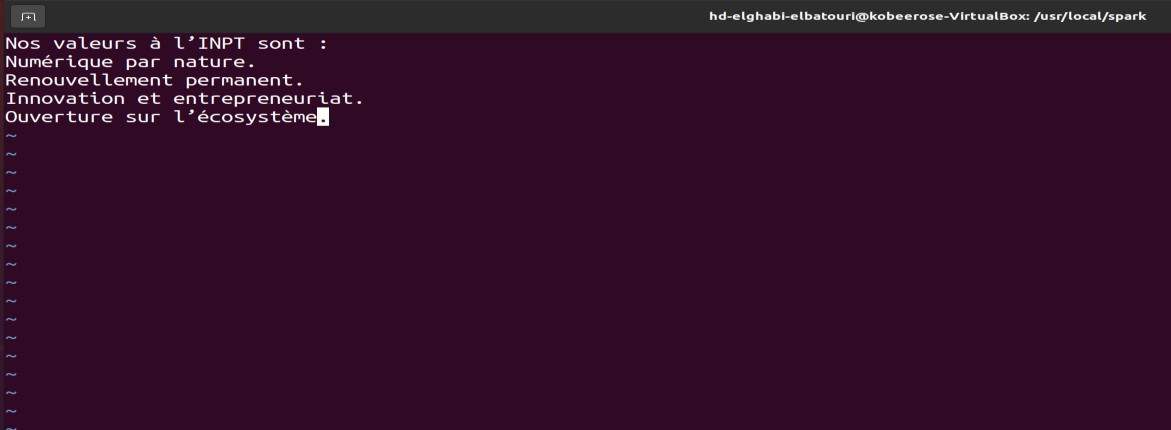
\includegraphics[width=1\linewidth]{Big_Data/Spark/Manipulating RDDs using pyspark/Creating ValeursINPT file.jpg} 
\end{center} 
\caption{caption} 
\end{figure} 
\FloatBarrier



\par Loading the files to pyspark.
\\
\begin{figure}[!htb] 
\begin{center} 
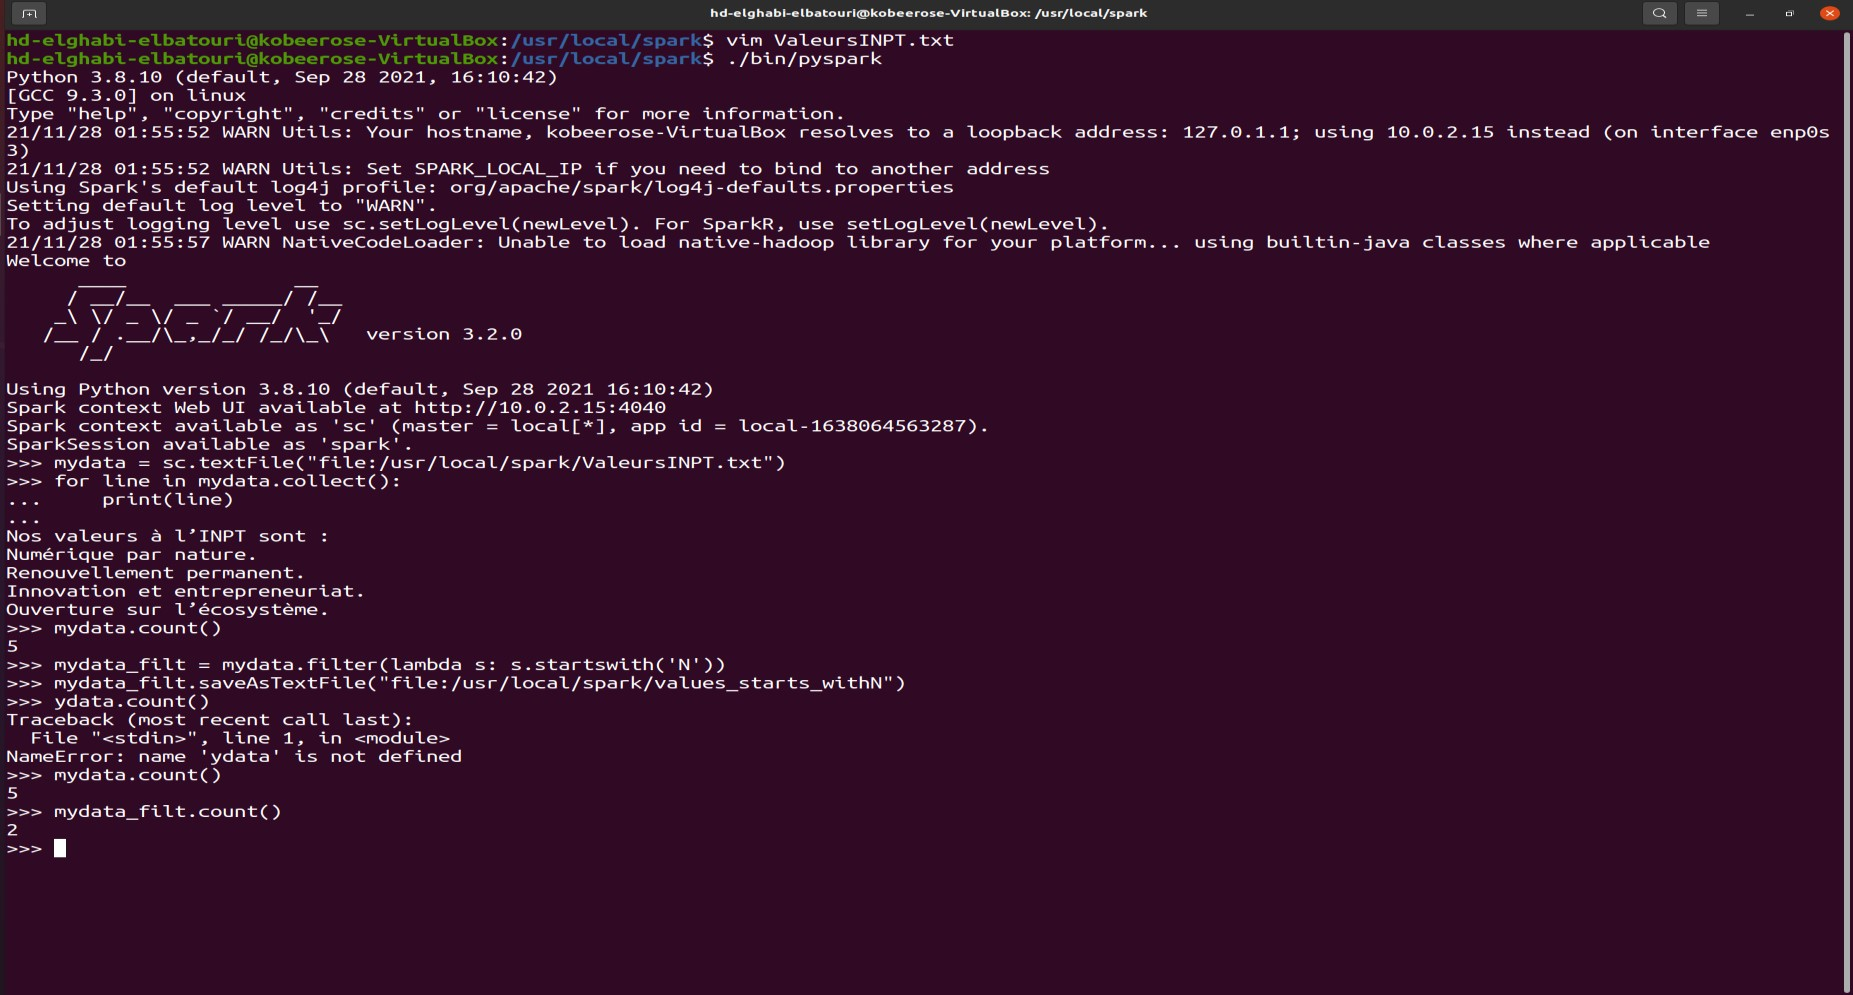
\includegraphics[width=1\linewidth]{Big_Data/Spark/Manipulating RDDs using pyspark/Loading file in pyspark.jpg} 
\end{center} 
\caption{caption} 
\end{figure} 
\FloatBarrier

\section{Loading SequenceFiles}

\par Loading and Saving RDD SequenceFiles using .saveAsSequenceFile command.
\\
\begin{figure}[!htb] 
\begin{center} 
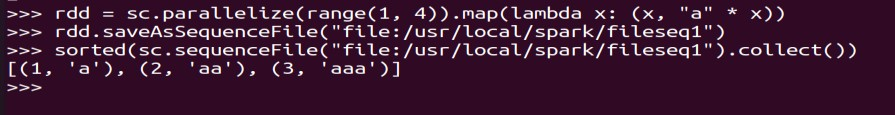
\includegraphics[width=1\linewidth]{Big_Data/Spark/Manipulating RDDs using pyspark/Loading Sequencefiles.jpg} 
\end{center} 
\caption{caption} 
\end{figure} 
\FloatBarrier

\section{Using functions}

\par We could be using both named and anonymous ( Lambda ) functions.
\\
\begin{figure}[!htb] 
\begin{center} 
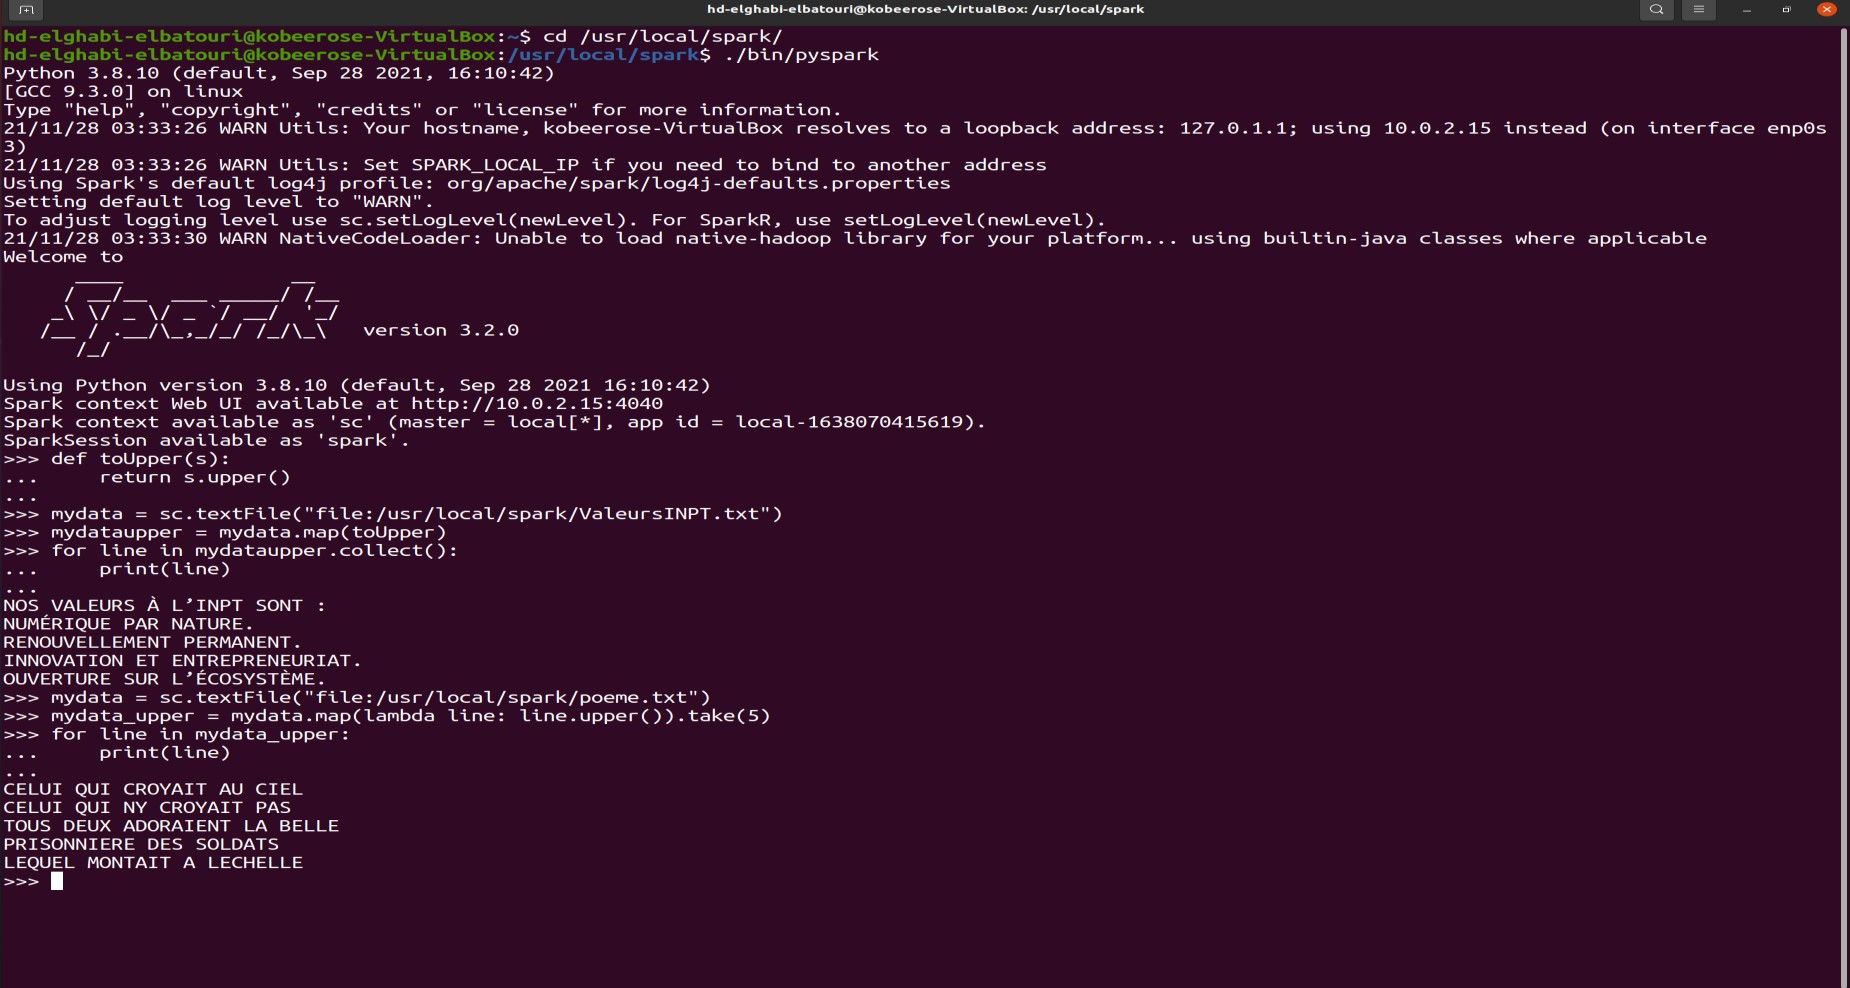
\includegraphics[width=1\linewidth]{Big_Data/Spark/Manipulating RDDs using pyspark/Using Functions.jpg} 
\end{center} 
\caption{caption} 
\end{figure} 
\FloatBarrier

\section{Working with Json}


\par First in the /usr/local/spark directory, we make a directory named: json_files and which we create two json files to play with.
\\
\begin{figure}[!htb] 
\begin{center} 
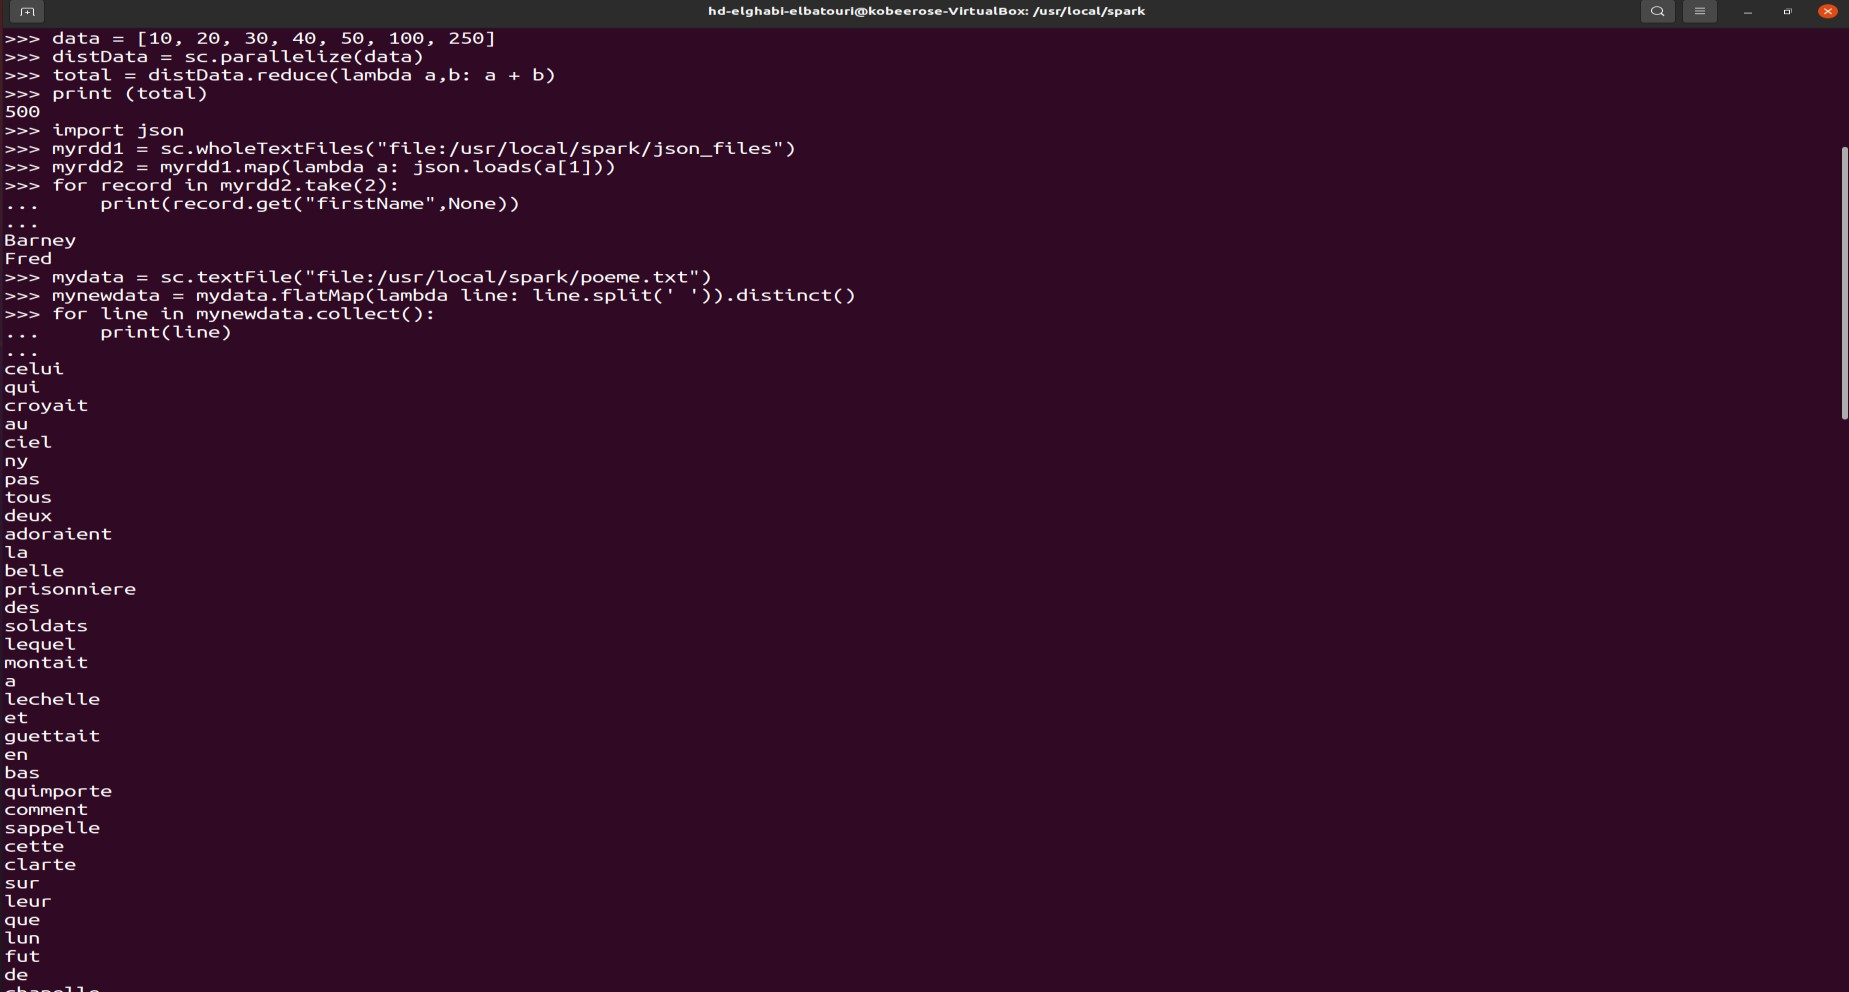
\includegraphics[width=1\linewidth]{Big_Data/Spark/Manipulating RDDs using pyspark/Working with Json.jpg} 
\end{center} 
\caption{caption} 
\end{figure} 
\FloatBarrier

\section{Intersection and union}

\par Let's try using intersection and union methods.
\\
\begin{figure}[!htb] 
\begin{center} 
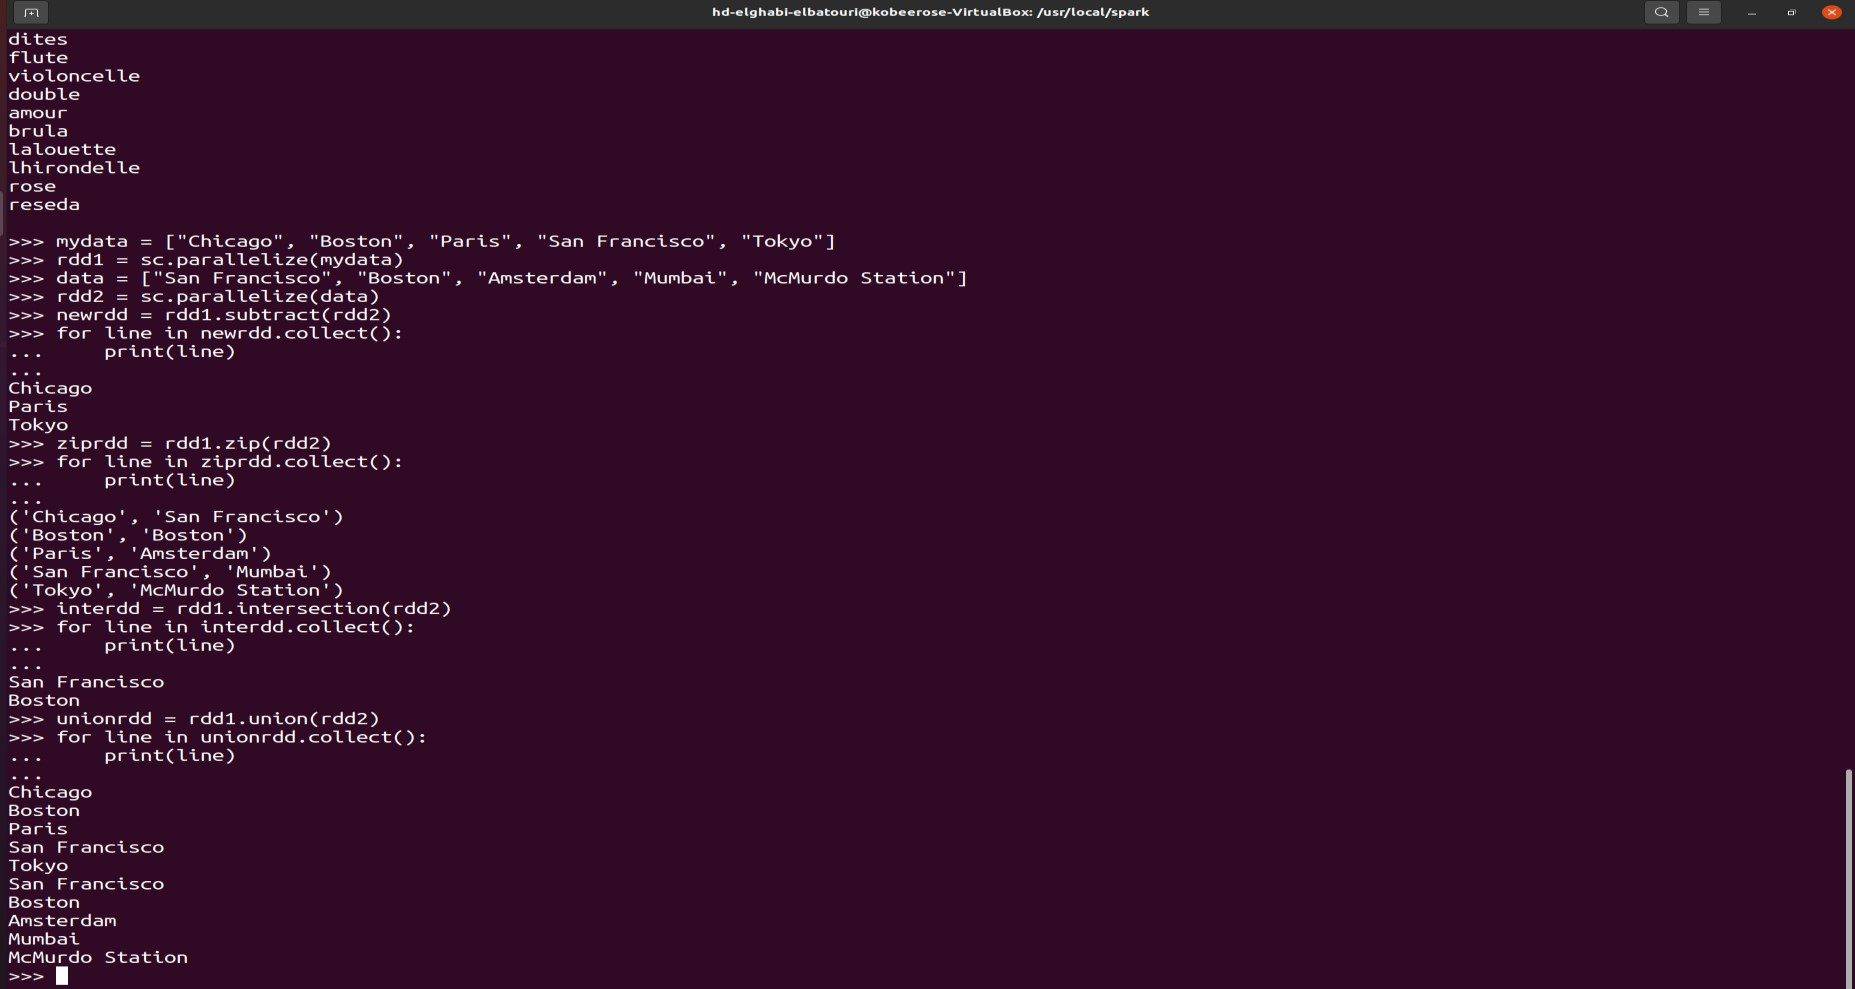
\includegraphics[width=1\linewidth]{Big_Data/Spark/Manipulating RDDs using pyspark/Intersection and union.jpg} 
\end{center} 
\caption{caption} 
\end{figure} 
\FloatBarrier


\FloatBarrier

\end{spacing}